\documentclass[11pt]{beamer}
\usetheme{Antibes}
\usepackage{amsmath, amssymb}
\usepackage{ragged2e}
\usepackage {tikz}
\usetikzlibrary{positioning}
\usepackage {xcolor}
\definecolor {processblue}{cmyk}{0.96,0,0,0}
\title{FTechAI Training}
\subtitle{Using Beamer}
\author{Luc Nguyen}
\institute{HUST}
\date{\today}
\usetheme{Boadilla}

\begin{document}
\begin{frame}
	\frametitle{\textbf{OVER-FITTING}}
%	\framesubtitle{Introduction} % Fundamental principles Pros - Cons - Model
	\begin{itemize}
		\item Basic concepts
		\item Definition.% , underfiting and a good fit
		\item How to limit overfitting
		%\item Summary
	\end{itemize}
\end{frame}
\begin{frame}
	\frametitle{\textbf{OVER-FITTING}}
	\framesubtitle{Basic Concepts}
	\Large{Generalization of Machine Learning:}
	\begin{itemize}
		\item Try to predict the future event (output) $Y$ from the present events (input) $X$.
		\item General model :  $Y = f(X)$.
		\item Need to find function $f$ from training data set $Y$ and $X$, respectively.
	\end{itemize}
\end{frame}
\begin{frame}
	\frametitle{\textbf{OVER-FITTING}}
	\framesubtitle{Basic Concepts}
	\begin{minipage}{0.5\textwidth}
		\Large{Three posibilities of function $f$:}
		\begin{itemize}
			\item Good fit
			\item Under-fitting
			\item {\only<2>{\color{red}}Over-fitting} {\only<2>{: Studying likes a parrot}}
		\end{itemize}
	\end{minipage}
	\begin{minipage}{0.4\textwidth}
		\begin{flushright}
			\only<2>{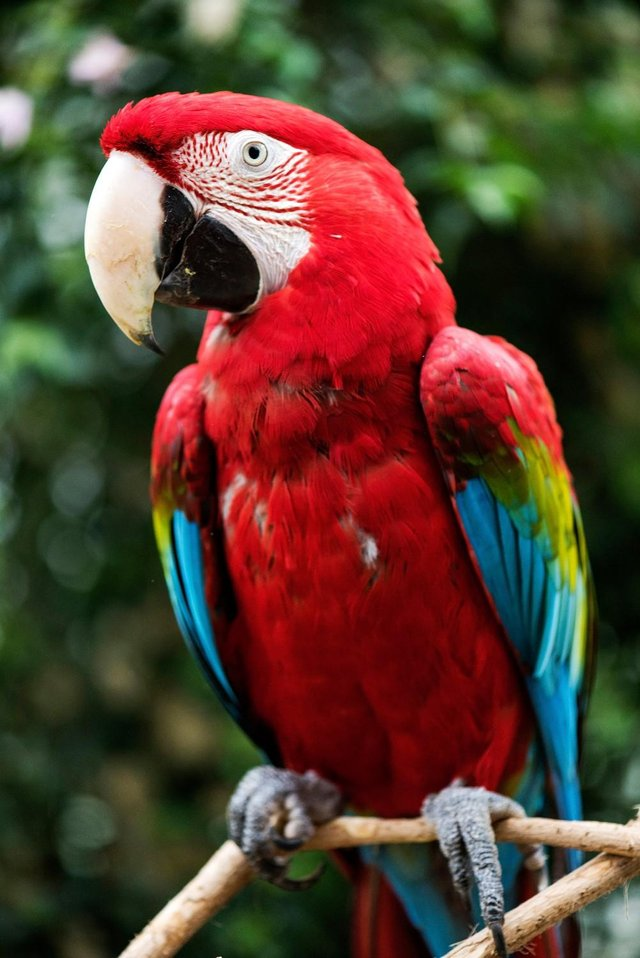
\includegraphics[scale=0.18]{parrot.jpg}}
		\end{flushright}
	\end{minipage}
\end{frame}
\begin{frame}
	\begin{center}
		\vspace*{\fill}
			\Huge{\textbf{\color{red}OVER-FITTING}}
		\vspace*{\fill}
	\end{center}
\end{frame}

% start graph
\begin{frame}
\begin{center}
	\frametitle{\textbf{OVER-FITTING}}
	\framesubtitle{Definition}
	\begin{tikzpicture}[domain=0:8, scale=0.6]
%\draw[thin,color=gray!50] (-0.9,-0.9) grid (7.9,5.9);
\draw[->] (-0.2,2) -- (8.2,2) node[right] {$x$};
\draw[->] (0,1.0) -- (0,8.2) node[above] {$f(x)$};
\foreach \Point in {(1, 3.741), (2, 4.509)}{
    \node at \Point {\textbullet};
}
\pause
\draw[color=blue, domain=0:7] plot(\x, {\x*0.7678 + 2.9736}) node[right] {$y = ax + b$};
\pause
\foreach \Point in {(3, 4.2411), (4, 3.643), (6, 4.120)}{
    \node at \Point {\textbullet};
}
	\end{tikzpicture}
\end{center}
\end{frame}


\begin{frame}
\begin{center}
	\frametitle{\textbf{OVER-FITTING}}
	\framesubtitle{Definition}
	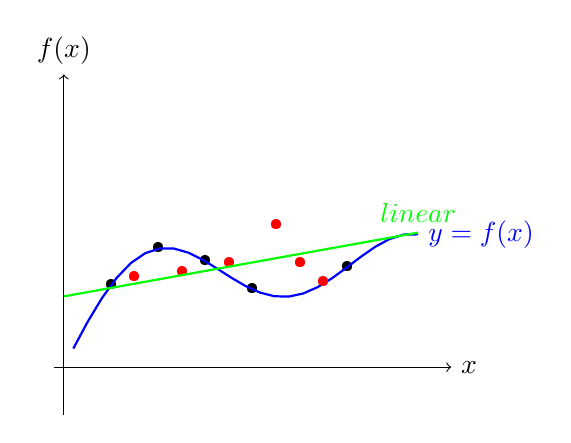
\begin{tikzpicture}[domain=0:8, scale=0.6]
%\draw[thin,color=gray!50] (-0.9,-0.9) grid (7.9,5.9);
\draw[->] (-0.2,2) -- (8.2,2) node[right] {$x$};
\draw[->] (0,1.0) -- (0,8.2) node[above] {$f(x)$};
\foreach \Point in {(1, 3.741), (2, 4.509), (3, 4.2411), (4, 3.643), (6, 4.120) }{
    \node at \Point {\textbullet};
}
\draw[color=blue, thick, domain=0.2:7.5] plot(\x,{-\x^2/10+\x+2+sin(\x r)}) node[right] {$y = f(x)$} ;
%\pause
\foreach \Point in {(1.5, 3.9), (2.5, 4), (3.5, 4.2), (4.5, 5), (5, 4.2), (5.5, 3.8) }{
    \node at \Point {\color{red}\textbullet};
}
\pause
\draw[color=green, thick, domain=0:7.5] plot(\x, {\x*0.18 + 3.5}) node[right, above] {$linear$};


	\end{tikzpicture}
\end{center}
\end{frame}

\iffalse
\begin{frame}
	\frametitle{\textbf{OVER-FITTING}}
	\framesubtitle{How to limit overfitting}
	\begin{itemize}
		\item Reduce the network's capacity
		\item Apply regularization
		\item Add dropout layers
	\end{itemize}
\end{frame}
\fi
\begin{frame}
	\frametitle{\textbf{OVER-FITTING}}
	\framesubtitle{How to limit overfitting}
	\begin{description}
		\item[\color{black}\textbf{Reduce the network's capacity}] remove layers or reduce the number of elements in the hidden layers.
	\end{description}
\end{frame}
\begin{frame}
	\frametitle{\textbf{OVER-FITTING}}
	\framesubtitle{How to limit overfitting}
	\begin{description}
		\item[\color{black}\textbf{Reduce the network's capacity}] remove layers or reduce the number of elements in the hidden layers.
		\item[\color{black}\textbf{Apply regularization}] add a cost to the loss function for large weights.
	\end{description}	
\end{frame}
\begin{frame}
	\frametitle{\textbf{OVER-FITTING}}
	\framesubtitle{How to limit overfitting}
	\begin{description}
		\item[\color{black}\textbf{Cross-validation}]
		\item[\color{black}\textbf{Reduce the network's capacity}] Remove layers or reduce the number of elements in the hidden layers.
		\item[\color{black}\textbf{Apply regularization}] Add a cost to the loss function for large weights.
		\item[\color{black}\textbf{Add dropout layers}] Randomly remove certain features by setting them to zero.
	\end{description}
	\pause
	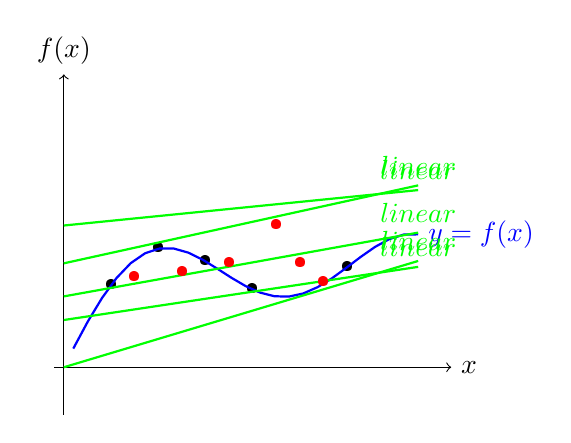
\begin{tikzpicture}[domain=0:8, scale=0.6]
%\draw[thin,color=gray!50] (-0.9,-0.9) grid (7.9,5.9);
\draw[->] (-0.2,2) -- (8.2,2) node[right] {$x$};
\draw[->] (0,1.0) -- (0,8.2) node[above] {$f(x)$};
\foreach \Point in {(1, 3.741), (2, 4.509), (3, 4.2411), (4, 3.643), (6, 4.120) }{
    \node at \Point {\textbullet};
}
\draw[color=blue, thick, domain=0.2:7.5] plot(\x,{-\x^2/10+\x+2+sin(\x r)}) node[right] {$y = f(x)$} ;
%\pause
\pause
\draw<1>[color=green, thick, domain=0:7.5] plot(\x, {\x*0.3 + 2}) node[right, above] {$linear$};
\draw<2>[color=green, thick, domain=0:7.5] plot(\x, {\x*0.1 + 5}) node[right, above] {$linear$};
\draw<3>[color=green, thick, domain=0:7.5] plot(\x, {\x*0.22 + 4.2}) node[right, above] {$linear$};
\draw<4>[color=green, thick, domain=0:7.5] plot(\x, {\x*0.15 + 3}) node[right, above] {$linear$};
\draw<5-6>[color=green, thick, domain=0:7.5] plot(\x, {\x*0.18 + 3.5}) node[right, above] {$linear$};

\foreach \Point in {(1.5, 3.9), (2.5, 4), (3.5, 4.2), (4.5, 5), (5, 4.2), (5.5, 3.8) }{
    \node<6> at \Point {\color{red}\textbullet};
}
	\end{tikzpicture}	
\end{frame}

%
%
%
%
% end graph
\iffalse
\begin{frame}
\begin{center}
	\frametitle{\textbf{OVER-FITTING}}
	\framesubtitle{How to limit overfitting}
	\begin{tikzpicture}[domain=0:8, scale=0.6]
%\draw[thin,color=gray!50] (-0.9,-0.9) grid (7.9,5.9);
\draw[->] (-0.2,2) -- (8.2,2) node[right] {$x$};
\draw[->] (0,1.0) -- (0,8.2) node[above] {$f(x)$};
\foreach \Point in {(1, 5/2), (2, 3), (3.5, 1.875)}{
    \node at \Point {\textbullet};
}
%\pause
\draw[color=blue, domain=0:4.7] plot(\x, -\x^2/2 + 2*\x + 1) node[right] {$y = ax^2 + bx + c$};
\node at (3.5, 1.875)  {\textbullet};

	\end{tikzpicture}
	
\end{center}
\end{frame}
\fi




\end{document}